\documentclass[compress, 8pt]{beamer}
% \documentclass[handout, 8pt]{beamer}
\usepackage[utf8]{inputenc}

% Notes to self: \nts[color option]{text that is a note}
\newif\ifshowcomments
% \showcommentstrue % uncomment to show
\input{preambleB}
\usepackage[normalem]{ulem}

%%%%%%%%%%%%%%%%%%%%%%%%%%%%%%%%%%%%%%%%%%%%%%%%%%%%%%%%%%%%%%%%%%%%%%%%%%%%%%
% Paths to figures
\usepackage{subcaption}

% Avoid a warning on mac; can introduce a warning (and maybe a break) on windows
% \usepackage{etex}
% Avoid a warning
\let\Tiny=\tiny

%Information to be included in the title page:
\title{Fixed effects and Differences-in-differences}
\subtitle{ECON726}
\author[]{Tara Sullivan}
\institute{
Tara Sullivan \\
\textit{tara.sullivan55@login.cuny.edu}
}
\date{
\today
\nts{\\
\medskip
Notes/comments are in gray and will be excluded from the presentation.
}
}

% plot graphs with pgfplots
\usepackage{pgfplots}
\pgfplotsset{compat=newest}
\usepgfplotslibrary{groupplots}
\usepgfplotslibrary{dateplot}
\pgfplotsset{compat=newest,
    every axis/.style={
        axis y line*=left,
        axis x line*=bottom,
        % allows for multi-line legend entries
        legend style={cells={align=left}},
        % allows for multi-line titles
        title style={align=center},
    },
}

% For animations using underbrace 
% Source: https://tex.stackexchange.com/a/565866
\usepackage{xparse, letltxmacro}
\LetLtxMacro{\oldunderbrace}{\underbrace}
\DeclareDocumentCommand{\underbrace}{d<> m e{_}}{%
  \IfValueTF{#1}{% IF <overlay-specification> given
    % using global onlside flag, cf. p82 beamer manual v3.59
    \oldunderbrace{#2\onslide<#1>}_{#3}\onslide%
  }{% ELSE
    \oldunderbrace{#2}_{#3}
  }%
}%

\usetikzlibrary{decorations.pathreplacing,calligraphy}

%%%%%%%%%%%%%%%%%%%%%%%%%%%%%%%%%%%%%%%%%%%%%%%%%%%%%%%%%%%%%%%%%%%%%%%%%%%%%%%%
\begin{document}    
%\beamertemplatenavigationsymbolsempty


%%%%%%%%%%%%%%%%%%%%%%%%%%%%%%%%%%%%%%%%%%%%%%%%%%%%%%%%%%%%%%%%%%%%%%%%%%%%%%%%
\begin{frame}
\titlepage
% \tikzset{external/figure name={intro_}}
\end{frame}

%%%%%%%%%%%%%%%%%%%%%%%%%%%%%%%%%%%%%%%%%%%%%%%%%%%%%%%%%%%%%%%%%%%%%%%%%%%%%%%%
\begin{frame}{Housekeeping}

Agenda:
\begin{itemize}
    \item Discuss project plans
    \item Discuss next assignment: replication results
    \item Fixed effects and differences-in-differences
\end{itemize}

Homework:
\begin{itemize}
    \item There will be a short homework assignment this week (graded for completion), asking you to describe the conditional independence assumption in your own words, and why that matters for causal inference
    \begin{itemize}
        \item You will need to do something like this in your final paper, so please put in the effort!
    \end{itemize}
    \item If you haven't, \textbf{run your code}
    \begin{itemize}
        \item You should be working on distilling your code to \emph{only} key results/what will be in your final paper
    \end{itemize}

    \item Reading: 
    \begin{itemize}
        \item Cunningham Chp. 10: \url{https://mixtape.scunning.com/10-synthetic_control}
        \item I'll likely also use code from here: \url{https://matheusfacure.github.io/python-causality-handbook/15-Synthetic-Control.html}
    \end{itemize}
\end{itemize}

\end{frame}

%%%%%%%%%%%%%%%%%%%%%%%%%%%%%%%%%%%%%%%%%%%%%%%%%%%%%%%%%%%%%%%%%%%%%%%%%%%%%%%%
\begin{frame}{Empirical project}

\textbf{Paper selection}: Due \textbf{September 22} [5\% of final grade]
\begin{itemize}
\item Done! 
\end{itemize}

\textbf{Project plan}: Due \textbf{October 14} [15\% of final grade] 
\begin{itemize}
\item Done!
\end{itemize} 

\textbf{Replication results}: \textbf{November 3}: [10\% of final grade]
\begin{itemize}
\item You should submit some of your main replication results. The final results should be formatted as tables and charts in a word document or PDF, submitted on Brightspace. Your code and data should accessible on GitHub.
\end{itemize}

\textbf{Presentation}: Due \textbf{December 2} \& \textbf{December 9} [10\% of final grade]
\begin{itemize}
\item Prepare a \textbf{5-8} minute presentation on your paper. Focus on the research question, main result, and one extension. 
\end{itemize}

\textbf{Final Paper}: Due \textbf{December 16} [35\% of final grade]
\begin{itemize}
\item Your paper should contain \sout{5-8 pages} \textbf{6-10 pages} of text, and \sout{5-8 pages} \textbf{3-6 pages} of figures (double spaced, 12 point font).
You must provide the code and data to replicate your findings. 
Your final project should be submitted on Brightspace, and your code and data should be uploaded to github (note: if your data is too large to upload to github, let me know). 
\end{itemize}

\end{frame}

%%%%%%%%%%%%%%%%%%%%%%%%%%%%%%%%%%%%%%%%%%%%%%%%%%%%%%%%%%%%%%%%%%%%%%%%%%%%%%%%
\begin{frame}{Project plans}

General feedback:
\begin{itemize}
    \item \textbf{These were generously graded}. I wanted to give people credit for staying on track.
    \begin{itemize}
        \item 17/20: \textbf{Your plan is sufficient, but your project needs work}
        \item 20/20: You're on track, but you still may need to address issues
    \end{itemize}
\end{itemize}
\textbf{Read the comments on your assignment!}

\vspace{3ex}
Overall feedback: 
\begin{itemize}
    \item For your final paper, you need to motivate why your method is causal. The authors will say "I use differences-in-differences to identify..." You cannot get away with that. You need to motivate why yor method is causal. If you don't discuss the conditional independence assumption, you will lose a lot of points. \textbf{This will be graded harshly on your final project}
    
    \begin{itemize}
        \item Part of that will include discussing what the ideal randomized experiment is. 
        \item You need to explain why this method is causal
    \end{itemize}

    \item Do \textbf{NOT} reference methodologies that you cannot explain why they are important. 

    \begin{itemize}
        \item These are long, published papers. If you cannot explain in plain language the robustness check, don't include it. 
    \end{itemize}

    \item You're expected to incorporate parts of the reading into your discussion of causality (and, likely, do readings from secondary sources)
\end{itemize}

\end{frame}

%%%%%%%%%%%%%%%%%%%%%%%%%%%%%%%%%%%%%%%%%%%%%%%%%%%%%%%%%%%%%%%%%%%%%%%%%%%%%%%%
\begin{frame}{Next assignments: replication and presentation}

You are expected to replicate key results. 
\begin{itemize}
    \item If you simply upload the replication file for the paper, you will fail
    \item You need to distill these files to only \textbf{key results}
    \item I should effectively do \textbf{zero} data cleaning when I re-run your files. You should have a clean file, a few lines of code; that's it
\end{itemize}

\vspace{2ex}
When replicating your results, keep in mind your presentation.
\begin{itemize}
    \item Your presentation can only be about 3-4 slides. 
    \begin{enumerate}
        \item 1 slide with intro/context/question
        \item 1-2 slide on key points of data/methodology
        \item 1-2 slide with key results
        \item 0-1 slide with extension
    \end{enumerate}
\end{itemize}
How do you distill this paper to key takeaways?
\end{frame}





%%%%%%%%%%%%%%%%%%%%%%%%%%%%%%%%%%%%%%%%%%%%%%%%%%%%%%%%%%%%%%%%%%%%%%%%%%%%%%%
\miniframesoff
\begin{frame}{Outline}
    \tableofcontents
\end{frame}
\miniframeson



%%%%%%%%%%%%%%%%%%%%%%%%%%%%%%%%%%%%%%%%%%%%%%%%%%%%%%%%%%%%%%%%%%%%%%%%%%%%%%%%
\section[Fixed effects]{Fixed effects}
\miniframesoff
\begin{frame}
    \tableofcontents[currentsection]
\end{frame}
\miniframeson
%%%%%%%%%%%%%%%%%%%%%%%%%%%%%%%%%%%%%%%%%%%%%%%%%%%%%%%%%%%%%%%%%%%%%%%%%%%%%%%%

%%%%%%%%%%%%%%%%%%%%%%%%%%%%%%%%%%%%%%%%%%%%%%%%%%%%%%%%%%%%%%%%%%%%%%%%%%%%%%%%
\begin{frame}{Intro}

Key to causal inference in Chapter 3 of MHE is to control for confounding factors
\begin{itemize}
    \item What if the confounding variables are unobservable?
\end{itemize}

Today: control for unobserved variables that are fixed by time or by cohort
\begin{itemize}
    \item Fixed effects
    \item Differences-in-differences
\end{itemize}

\end{frame}


%%%%%%%%%%%%%%%%%%%%%%%%%%%%%%%%%%%%%%%%%%%%%%%%%%%%%%%%%%%%%%%%%%%%%%%%%%%%%%%%
\begin{frame}{Motivating example}

Define
\begin{itemize}
    \item $Y_i$: the (log) wages of individual $i$
    \item $D_i$: Union membership
\end{itemize}
Does collective bargaining increase wages? Or would those workers have earned more anyway, perhaps because they because are more experienced or skilled?

\vspace{3ex}
Slight change to potential outcomes notation: $Y_{di}$ will now be $Y_i (d)$
\begin{itemize}
    \item $Y_{1i}$ will now be $Y_i (1)$
    \begin{itemize}
        \item Treatment potential outcome
        \item The value of $Y_i$ under treatment, irrespective of whether $i$ was treated
        \item Wages for $i$ if unionized, irrespective of whether they were in a union
    \end{itemize}
    \item $Y_{0i}$ will now be $Y_i (0)$
    \begin{itemize}
        \item Control potential outcome
        \item Wages for $i$ if not unionized, irrespective of $i$ was in a union
    \end{itemize}
\end{itemize}

\end{frame}

%%%%%%%%%%%%%%%%%%%%%%%%%%%%%%%%%%%%%%%%%%%%%%%%%%%%%%%%%%%%%%%%%%%%%%%%%%%%%%%%
\begin{frame}{Time dimension}

Adding a time dimension to our outcome variable and treatment:
\begin{itemize}
    \item $Y_{it}$: observed (log) wages of individual $i$ at time $t$
    \item $D_{it}$: union membership of individual $i$ at time $t$
    \item $X_{it}$: observed, time-varying covariates
    \item $A_i$: \textbf{unobserved but fixed} confounders
    \begin{itemize}
         \item Assume $A_i$ is an individual's innate ability, and is fixed over time
         \item $A_i$ should include all other time-invariant characteristics, like biological sex
     \end{itemize} (for example, ability of individual $i$)
\end{itemize}
Potential outcomes: $Y_{it}(d)$
\begin{itemize}
    \item $Y_{it} (0)$: Control potential outcome 
    \item $Y_{it} (1)$: Treatment potential outcome
\end{itemize}

\end{frame}

%%%%%%%%%%%%%%%%%%%%%%%%%%%%%%%%%%%%%%%%%%%%%%%%%%%%%%%%%%%%%%%%%%%%%%%%%%%%%%%%
\begin{frame}{}

Assume conditional independence holds:
\begin{equation*}
    \EE [Y_{it} (0) \vert A_i, X_{it}, t, D_{it}] = \EE [Y_{it} (0) \vert A_i, X_{it}, t]
\end{equation*}
\begin{itemize}
    \item Union membership is as good as randomly assigned conditional on $A_i$, and observed covariates 
\end{itemize}
 Assume a linear model for $\EE [Y_{it} (d) \vert \cdot]$, where $A_i$ does not have a time subscript:
 \begin{equation*}
     \EE [Y_{it} (0) \vert A_i, X_{it}, t] 
     = \alpha + \lambda_t + A_i^\prime \gamma + X^\prime \beta
 \end{equation*}
Assume the causal effect of union membership is a constant, $\rho$:
\begin{equation*}
    \EE [Y_{it} (1) \vert A_i, X_{it}, t] = \EE[Y_{it} (0) \vert A_i, X_{it}, t]  + \rho
\end{equation*}
The above equations imply:
\begin{equation*}
    \EE [Y_{it} \vert A_i, X_{it}, t, D_{it}] = \alpha + \lambda_t + \rho D_{it} + A_i^\prime \gamma + X_{it}^\prime \beta
\end{equation*}
Note: these are more restrictive assumptions than we used in previous sections; we are explictly assuming a linear, additive functional form 

\end{frame}

%%%%%%%%%%%%%%%%%%%%%%%%%%%%%%%%%%%%%%%%%%%%%%%%%%%%%%%%%%%%%%%%%%%%%%%%%%%%%%%%
\begin{frame}{}

Fixed effects model: 
\begin{equation*}
    Y_{it} = \alpha_i + \lambda_t + \rho D_{it} + X_{it}^\prime \beta + \epsilon_{it},
\end{equation*}
where:
\begin{equation*}
    \epsilon_{it} \equiv Y_{it} (0) - \EE [Y_{it} (0) \vert A_i, X_{it}, t], \quad \alpha_i = \alpha + A_i^\prime \gamma
\end{equation*}

\vspace{3ex}
\begin{itemize}
    \item Causal effect of treatment (i.e. union status on wages) is given by $\rho$
    \item Individual fixed effects $\alpha_i$ is a parameter to be estimated
    \begin{itemize}
        \item Given by coefficients on dummies for each individual
    \end{itemize}
    \item Time fixed effects $\lambda_t$ is a parameter to be estimated
    \begin{itemize}
        \item Given by coefficient on dummies for each time period in the model
    \end{itemize}
\end{itemize}

\vspace{3ex}
Important notes:
\begin{itemize}
    \item Each element of $X_{it}$ must vary across time for each cross-section $i$
\end{itemize}

\end{frame}

%%%%%%%%%%%%%%%%%%%%%%%%%%%%%%%%%%%%%%%%%%%%%%%%%%%%%%%%%%%%%%%%%%%%%%%%%%%%%%%%
\begin{frame}{}

Fixed effects: estimate a coefficient for a dummy on each individual $i$
\begin{itemize}
    \item This could be a big computational lift
    \begin{itemize}
        \item Example: estimating effect of union membership on wages
        \item Might use Panel Survey of Income Dynamics (PSID) data, with data on 5,000 men ($N=5,000$) observed for 20 years ($T=20$)
        \item Estimating coefficients on 4,999 individuals seems computational difficult
    \end{itemize}
    \item In practice, you don't need to estimate all coefficients
\end{itemize}

\vspace{3ex}


\end{frame}


%%%%%%%%%%%%%%%%%%%%%%%%%%%%%%%%%%%%%%%%%%%%%%%%%%%%%%%%%%%%%%%%%%%%%%%%%%%%%%%%
\begin{frame}{}

Consider equation with only individual fixed effects:
\begin{equation*}
    Y_{it} = \alpha_i + \rho D_{it} + X_{it}^\prime \beta + \epsilon_{it}
\end{equation*}
Consider the average over all $t$ for individual $i$ e.g. $\bar{Y}_i = \sum_{t=1}^T Y_{it}$
\begin{equation*}
    \bar{Y}_i = \alpha_i + \rho \bar{D}_i + \bar{X}^\prime \beta + \bar{\epsilon}_i
\end{equation*}
Subtract the mean equation from the regression, we have the ``de-meaned'' regression:
\begin{align*}
    Y_{it} - \bar{Y}_i =& \alpha_i + \rho D_{it} + X_{it}^\prime \beta + \epsilon_{it} - \left( \alpha_i + \rho \bar{D}_i + \bar{X}^\prime \beta + \bar{\epsilon}_i \right) \\
    =& (\alpha_i - \alpha_i) 
    + \rho (D_{it} - \bar{D}_i)
    + (X_{it} - \bar{X}_i)^\prime \beta 
    + (\epsilon_{it} - \bar{\epsilon}_i) \\
    =& \rho (D_{it} - \bar{D}_i)
    + (X_{it} - \bar{X}_i)^\prime \beta 
    + (\epsilon_{it} - \bar{\epsilon}_i) \\
    \ddot{Y}_{it} =& \rho \ddot{D}_{it}
    + \ddot{X}_{it}^\prime \beta 
    + \ddot{\epsilon}_{it}
\end{align*}
Can estimate $\rho$ from the de-meaned data; much more computationally simple!
\begin{itemize}
    \item Deviations from the mean kill individual fixed effects
    \item Fixed effects estimator often called the ``within'' estimator; 
\end{itemize}

\end{frame}

%%%%%%%%%%%%%%%%%%%%%%%%%%%%%%%%%%%%%%%%%%%%%%%%%%%%%%%%%%%%%%%%%%%%%%%%%%%%%%%%
\begin{frame}{First differences}

An alternative to de-meaning is to estimate first differences. Let $\Delta Y_{it} = Y_{it} - Y_{it-1}$:
\begin{align*}
    \Delta Y_{it} =& Y_{it} - Y_{it-1} \\
    =& (\alpha_i - \alpha_i) + \rho (D_{it} - D_{it-1}) + (X_{it} - X_{it-1})^\prime \beta + (\epsilon_{it} - \epsilon_{it-1}) \\
    =& \rho \Delta D_{it} + \Delta X_{it}^\prime \beta + \Delta \epsilon_{it}
\end{align*}
When there are only 2 periods, the fixed effects and first differenced estimators will be identical.
    \begin{align*}
        Y_{i2} - \bar{Y}_i &= Y_{i2} - \frac{Y_{i2} - Y_{i1}}{2} \\
        &= \frac{2 Y_{i2} - Y_{i2} - Y_{i1}}{2} \\
        &= \frac{Y_{i2} - Y_{i1}}{2}
    \end{align*}
\begin{itemize}
    \item  The de-meaned data is proportional to the first-differenced data $\implies$ the fixed effect estimator is the same as the first-differenced estimator
\end{itemize}
When there are more than 2 periods, the fixed effects data is likely not equal to the first differenced estimator; this is because of correlation between $\epsilon_{it}$ and $X_{is}$

\end{frame}


%%%%%%%%%%%%%%%%%%%%%%%%%%%%%%%%%%%%%%%%%%%%%%%%%%%%%%%%%%%%%%%%%%%%%%%%%%%%%%%%
\begin{frame}{Fixed effects estimation}

Go through example here: \url{https://mixtape.scunning.com/08-panel_data}
\begin{itemize}
    \item Python code available on my github: \url{https://github.com/tara-sullivan/econ726-notebooks/blob/main/notebooks/07-panel.ipynb}
\end{itemize}

\end{frame}

% %%%%%%%%%%%%%%%%%%%%%%%%%%%%%%%%%%%%%%%%%%%%%%%%%%%%%%%%%%%%%%%%%%%%%%%%%%%%%%%%
% \begin{frame}{Fixed effects pitfalls}

% To do; I don't like the twin example in MHE
% % \begin{itemize}
% %     \item Fixed effects control for time-invariant omitted variables
% %     \item Sometimes economic variables of interest are mostly time invariant
% %     \begin{itemize}
% %         \item Union membership is largely constant and varies little yearly
% %         \item Changes in union membership might be driven 
% %     \end{itemize}
% % \end{itemize}

% \end{frame}


%%%%%%%%%%%%%%%%%%%%%%%%%%%%%%%%%%%%%%%%%%%%%%%%%%%%%%%%%%%%%%%%%%%%%%%%%%%%%%%%
\section[Diff-in-diff]{Differences-in-differences}
\miniframesoff
\begin{frame}
    \tableofcontents[currentsection]
\end{frame}
\miniframeson
%%%%%%%%%%%%%%%%%%%%%%%%%%%%%%%%%%%%%%%%%%%%%%%%%%%%%%%%%%%%%%%%%%%%%%%%%%%%%%%%

%%%%%%%%%%%%%%%%%%%%%%%%%%%%%%%%%%%%%%%%%%%%%%%%%%%%%%%%%%%%%%%%%%%%%%%%%%%%%%%%
\begin{frame}{Cholera example}

In mid-1800s London, cholera was spreading
\begin{itemize}
    \item Awful, often fatal disease
    \item At the time, doctors thought it spread through the air
    \item In fact, it spread through contaminated food and water supply
    \begin{itemize}
        \item Sewage, containing cholera from ill people, would flow into the Thames, which would contaminate the water supply, which would cause more cholera
    \end{itemize}
\end{itemize}

Researcher John Snow suspected that it may be the water supply causing cholera transmission
\begin{itemize}
    \item Several water companies served different areas of the city
    \item In 1849, the \textbf{Lambeth (L)} water company moved their pipes upstream, above the main sewage discharge point
    \item The \textbf{Southwark and Vauxhall (SV)} Waterworks Company served similar households to the Lambeth Company, and did not move their intake point upstream
\end{itemize}
Snow evaluated one of the earliest \textbf{natural experiments}

\end{frame}

%%%%%%%%%%%%%%%%%%%%%%%%%%%%%%%%%%%%%%%%%%%%%%%%%%%%%%%%%%%%%%%%%%%%%%%%%%%%%%%%
\begin{frame}{Cross sectional comparison (fixed effects approach)}

Let:
\begin{itemize}
    \item $Y$: Outcome (cholera deaths)
    \item $D$: Treatment dummy (clean water)
    \item $L$: Lambeth fixed effect
    \item $SV$: Southwark and Vauxhall fixed effect
\end{itemize}
\begin{table}
\begin{tabular}{ll}
\textbf{Company} &\textbf{Outcome} \\
Lambeth & $Y = L + D$ \\
Southwark and Vauxhall & $Y = SV$
\end{tabular}
\end{table}
If estimated causal effect come from simple comparison of outcomes:
\begin{equation*}
    D + (L - SV)
\end{equation*}
We can think of $(L - SV)$ may contain selection bias

\end{frame}

%%%%%%%%%%%%%%%%%%%%%%%%%%%%%%%%%%%%%%%%%%%%%%%%%%%%%%%%%%%%%%%%%%%%%%%%%%%%%%%%
\begin{frame}{Pre-post comparison (interrupted time series; time fixed effect)}

Let:
\begin{itemize}
    \item $Y$: Outcome (cholera deaths)
    \item $D$: Treatment dummy (clean water)
    \item $L$: Lambeth fixed effect
    \item $T$: Time fixed effect
\end{itemize}
\begin{table}
\begin{tabular}{ll}
\textbf{Company} &\textbf{Outcome} \\
Lambeth before & $Y = L$ \\
Lambeth after & $Y = L + (T + D)$
\end{tabular}
\end{table}
If estimated causal effect come from simple comparison of outcomes:
\begin{equation*}
    L + (T + D) - L = T + D
\end{equation*}
\begin{itemize}
    \item Eliminates unit-specific fixed effect $L$
    \item $T$ isn't observable, so this can't be estimated
    \begin{itemize}
    \item This is both generally true, and specific to this example: cholera often arrived in waves
\end{itemize}
\end{itemize}




\end{frame}

%%%%%%%%%%%%%%%%%%%%%%%%%%%%%%%%%%%%%%%%%%%%%%%%%%%%%%%%%%%%%%%%%%%%%%%%%%%%%%%%
\begin{frame}{Difference-in-differences}

Let:
\begin{itemize}
    \item $D_1$: Pre/Post difference
    \item $D_2$: Cross-sectional difference
\end{itemize}
\begin{table}
\begin{tabular}{lllll}
\hline
\textbf{Company} &\textbf{Time} &\textbf{Outcome} &$D_1$ &$D_2$ \\
\hline\hline
Lambeth                &Before &$Y = L$            &\\
\hline
Lambeth                &After  &$Y = L + (T + D)$  &$T - D$ &$D$\\
\hline
Southwark and Vauxhall &Before &$Y = SV$           & \\
\hline
Southwark and Vauxhall &After  &$Y = SV + T$       &$T$ \\
\end{tabular}
\end{table}
\begin{itemize}
    \item The before-after difference eliminates the company fixed effects
    \item The difference in differences eliminates the time effects
\end{itemize}

\vspace{2ex}
Key assumption: \textbf{Parallel trends}
\begin{itemize}
    \item There is no time-variant company specific unobservables.
    \begin{itemize}
         \item $T$ is the same for all households
         \item Nothing unobserved in Lambeth households that is changing between these two periods that also determines cholera deaths
     \end{itemize} 
\end{itemize}
\end{frame}

%%%%%%%%%%%%%%%%%%%%%%%%%%%%%%%%%%%%%%%%%%%%%%%%%%%%%%%%%%%%%%%%%%%%%%%%%%%%%%%%
\begin{frame}{Diff-in-diff using potential outcomes}

Set-up:
\begin{itemize}
    \item Two groups (treatment and control): $G=1$ and $G=2$
    \item Two periods (before and after the treatment): $T=0$ and $T=1$
    \item Only one group is treated during one period
\end{itemize}

\vspace{2ex}
Using the potential outcomes framework:
\begin{itemize}
    \item $D$: treatment indicator, defined by $D = T \cdot G$
    \item $Y (d)$: potential outomce
    \item $Y$: observed outcome variable
    \begin{equation*}
        Y = D \cdot Y (1) + (1 - D) \cdot Y (0)
    \end{equation*}
\end{itemize}

\vspace{2ex}
\textbf{Key assumption: Common trends} $\EE [ Y(0) \vert G, T =1 ] - \EE [Y(0) \vert G, T= 0]$ does not depend on $G$



\end{frame}

%%%%%%%%%%%%%%%%%%%%%%%%%%%%%%%%%%%%%%%%%%%%%%%%%%%%%%%%%%%%%%%%%%%%%%%%%%%%%%%%
\begin{frame}{}

% \begin{align*}
% \EE [Y \vert D = 1] - \EE [Y \vert D=0] 
% % =& \EE [Y_1 \vert D=1] { - \EE [Y_0 \vert D = 1] + \EE [Y_0 \vert D = 1]}  - \EE [Y_0 \vert D=0] \\
% =& \underbrace{\EE [Y(1) - Y(0) \vert D = 1]}_{\text{ATE on treated}} 
% + \underbrace{\EE [Y(0) \vert D = 1] - \EE [Y(0) \vert D=0]}_{\text{Selection bias}}
% \end{align*}

% \begin{align*}
%     \EE [Y ]
% \end{align*}

Recall $Y = D \cdot Y (1) + (1 - D) \cdot Y (0)$ and {\color<3>{orange}$D = T \cdot G$}. The observed difference in differences is given by:
\begin{align*}
    &(\EE [{\color<2>{cyan} Y} \vert G = 1, T = 1] - \EE [{\color<2>{cyan}Y} \vert G = 1, T = 0])
    - (\EE [{\color<2>{cyan}Y} \vert G = 0, T = 1] - \EE [{\color<2>{cyan}Y} \vert G = 0, T = 0]) \\
    \only<2-4>{
    \onslide<2->{=& (
            \EE [{\color<2>{cyan} D Y(1) + (1 - D) Y(0)} \vert G = 1, T = 1] 
            - \EE [{\color<2>{cyan} D Y(1) + (1 - D) Y(0)} \vert G = 1, T = 0]
        ) \\
        & - (
            \EE [{\color<2>{cyan} D Y(1) + (1 - D) Y(0)} \vert G = 0, T = 1] 
            - \EE [{\color<2>{cyan} D Y(1) + (1 - D) Y(0)} \vert G = 0, T = 0]
        ) \\}
    \onslide<3->{=& (
            \EE [{{\color<3>{orange}TG} Y(1) + (1 - {\color<3>{orange}TG}) Y(0)} \vert G = 1, T = 1] 
            - \EE [{{\color<3>{orange}TG} Y(1) + (1 - {\color<3>{orange}TG}) Y(0)} \vert G = 1, T = 0]
        ) \\
        & - (
            \EE [{{\color<3>{orange}TG} Y(1) + (1 - {\color<3>{orange}TG}) Y(0)} \vert G = 0, T = 1] 
            - \EE [{{\color<3>{orange}TG} Y(1) + (1 - {\color<3>{orange}TG}) Y(0)} \vert G = 0, T = 0]
        ) \\}
    % \onslide<4->{=& (
    %         \EE [{1 Y(1) + (1 - {\color<4>{orange}1}) Y(0)} \vert G = 1, T = 1] 
    %         - \EE [{0 Y(1) + (1 - {\color<4>{orange}0}) Y(0)} \vert G = 1, T = 0]
    %     ) \\
    %     & - (
    %         \EE [{0 Y(1) + (1 - {\color<4>{orange}0}) Y(0)} \vert G = 0, T = 1] 
    %         - \EE [{0 Y(1) + (1 - {\color<4>{orange}0}) Y(0)} \vert G = 0, T = 0]
    %     ) \\}
    }  % end only
    \onslide<4->{=& (
            \EE [{Y(1)} \vert G = 1, T = 1] 
            - \EE [{Y(0)} \vert G = 1, T = 0]
        ) \\
        & - (
            \EE [{Y(0)} \vert G = 0, T = 1] 
            - \EE [{Y(0)} \vert G = 0, T = 0]
        ) \\}
    \onslide<5->{
    =& {\color<6>{cyan} \EE [{Y(1)} \vert G = 1, T = 1]} 
            {\color<6>{Green} - \EE [{Y(0)} \vert G = 1, T = 0]}
        ) \\
        & {\color<6>{Orange}- (
                    \EE [{Y(0)} \vert G = 0, T = 1] 
                    - \EE [{Y(0)} \vert G = 0, T = 0]
                )} \\
        & {\color<5>{red}
        {\color<6>{HunterPurple} + \EE [{Y(0)} \vert G = 1, T = 1]} 
        {\color<6>{MainBlue}- \EE [{Y(0)} \vert G = 1, T = 1]}}
    } \\
    \onslide<6->{
    =& 
        \underbrace{
            {\color<6>{cyan}\EE [{Y(1)} \vert G = 1, T = 1] }
            {\color<6>{MainBlue}- \EE [{Y(0)} \vert G = 1, T = 1]}
        }_{\text{ATT}} \\
        & \underbrace{{
                    {\color<6>{HunterPurple} + \EE [{Y(0)} \vert G = 1, T = 1]}
                    {\color<6>{Green} - \EE [{Y(0)} \vert G = 1, T = 0]}
                }}_{\text{Counterfactual difference for treated group}} \\
        & \underbrace{{\color<6>{Orange}- (
                            \EE [{Y(0)} \vert G = 0, T = 1] 
                            - \EE [{Y(0)} \vert G = 0, T = 0]
                        )}}_{\text{Difference for control}}
    }
\end{align*}
\end{frame}

%%%%%%%%%%%%%%%%%%%%%%%%%%%%%%%%%%%%%%%%%%%%%%%%%%%%%%%%%%%%%%%%%%%%%%%%%%%%%%%%
\begin{frame}{Parallel trends}

Observed differences in differences equals: 

\begin{multline*}
\underbrace{
            {\EE [{Y(1)} \vert G = 1, T = 1] }
            {- \EE [{Y(0)} \vert G = 1, T = 1]}
        }_{\text{ATT}} \\
        \underbrace{{
                    {+ \EE [{Y(0)} \vert G = 1, T = 1]}
                    { - \EE [{Y(0)} \vert G = 1, T = 0]}
                }}_{\text{Counterfactual difference for treated group}} \\
        \underbrace{{- (
                            \EE [{Y(0)} \vert G = 0, T = 1] 
                            - \EE [{Y(0)} \vert G = 0, T = 0]
                        )}}_{\text{Difference for control}}
\end{multline*}
For observed differences-in-differences to equal ATT, the latter half of this equation must equal zero:
\begin{multline*}
    \EE [{Y(0)} \vert G = 1, T = 1] - \EE [{Y(0)} \vert G = 1, T = 0] \\
    = \EE [{Y(0)} \vert G = 0, T = 1] - \EE [{Y(0)} \vert G = 0, T = 0]
\end{multline*}
This is known as the \textbf{parallel trends assumption}. If this doesn't equal zero, then bias is due to lack of parallel trends. 

\end{frame}

%%%%%%%%%%%%%%%%%%%%%%%%%%%%%%%%%%%%%%%%%%%%%%%%%%%%%%%%%%%%%%%%%%%%%%%%%%%%%%%%
\begin{frame}{Parallel trends (cont.)}

Suppose parallel trends holds:
\begin{align*}
    \alert{\EE [{Y(0)} \vert G = 1, T = 1] - \EE [{Y(0)} \vert G = 1, T = 0]} \\
    = \EE [{Y(0)} \vert G = 0, T = 1] - \EE [{Y(0)} \vert G = 0, T = 0]
\end{align*}
Consider the impact of a training program on earnings:
\begin{itemize}
    \item \alert{First term:} evolution of earnings for trainees had they not trained 
    \begin{itemize}
        \item This is fundamentally untestable
    \end{itemize}

    \item Evolution of mean earnings for non-trainees


\end{itemize}


\end{frame}



%%%%%%%%%%%%%%%%%%%%%%%%%%%%%%%%%%%%%%%%%%%%%%%%%%%%%%%%%%%%%%%%%%%%%%%%%%%%%%%%
\begin{frame}{Card and Krueger (1994)}

Setup: in Feb. 1992, NJ increased the state minimum wage from \$4.25 to \$5.05. PA minimum wage stayed at \$4.25
\begin{itemize}
    \item Two groups: treatment group ($G=1$) and control ($G=0$)
    \item Two periods: before ($T=0$) and after ($T=1$)
    \item Only one group is treated during one period
\end{itemize}

\vspace{2ex}
Data: survey of 400 fast food stores in NJ and PA before and after the minimum wage increase

\vspace{2ex}
Results: Card and Krueger (1994) find positive effects of increasing minimum wage on employment

\end{frame}



% %%%%%%%%%%%%%%%%%%%%%%%%%%%%%%%%%%%%%%%%%%%%%%%%%%%%%%%%%%%%%%%%%%%%%%%%%%%%%%%%
% \begin{frame}{}

% Using the potential outcomes framework:
% \begin{itemize}
%     \item $D$: treatment indicator, defined by $D = T \cdot G$
%     \item $Y (d)$: potential outomce
%     \item $Y$: observed outcome variable
%     \begin{equation*}
%         Y = D \cdot Y (1) + (1 - D) \cdot Y (0)
%     \end{equation*}
% \end{itemize}

% \vspace{2ex}
% \textbf{Key assumption: Common trends} $\EE [ Y(0) \vert G, T =1 ] - \EE [Y(0) \vert G, T= 0]$ does not depend on $G$



% \end{frame}



%%%%%%%%%%%%%%%%%%%%%%%%%%%%%%%%%%%%%%%%%%%%%%%%%%%%%%%%%%%%%%%%%%%%%%%%%%%%%%%%
\begin{frame}{}

Under parallel trends, differences in sample averages will estimate ATT

\vspace{2ex}
Researchers may want to use multivariate regression instead
\begin{itemize}
    \item Can help avoid omitted variable bias from endogenous covariates that vary over time
    \item By controlling for more appropriate covariates, you can reduce residual variance and improve the precision of your diff-in-diff estimate.
\end{itemize}

\vspace{2ex}
With constant state and time fixed effects, can estimate ATT from simple regression:
\begin{equation*}
    Y = \alpha + \gamma G + \lambda T + \delta (T \times G) + \epsilon
\end{equation*}

\end{frame}

%%%%%%%%%%%%%%%%%%%%%%%%%%%%%%%%%%%%%%%%%%%%%%%%%%%%%%%%%%%%%%%%%%%%%%%%%%%%%%%%
\begin{frame}{}

\begin{equation*}
    Y = \alpha + \gamma G + \lambda T + \delta (T \times G) + \epsilon
\end{equation*}

\begin{columns}
\begin{column}{.55\textwidth}
\begin{figure}
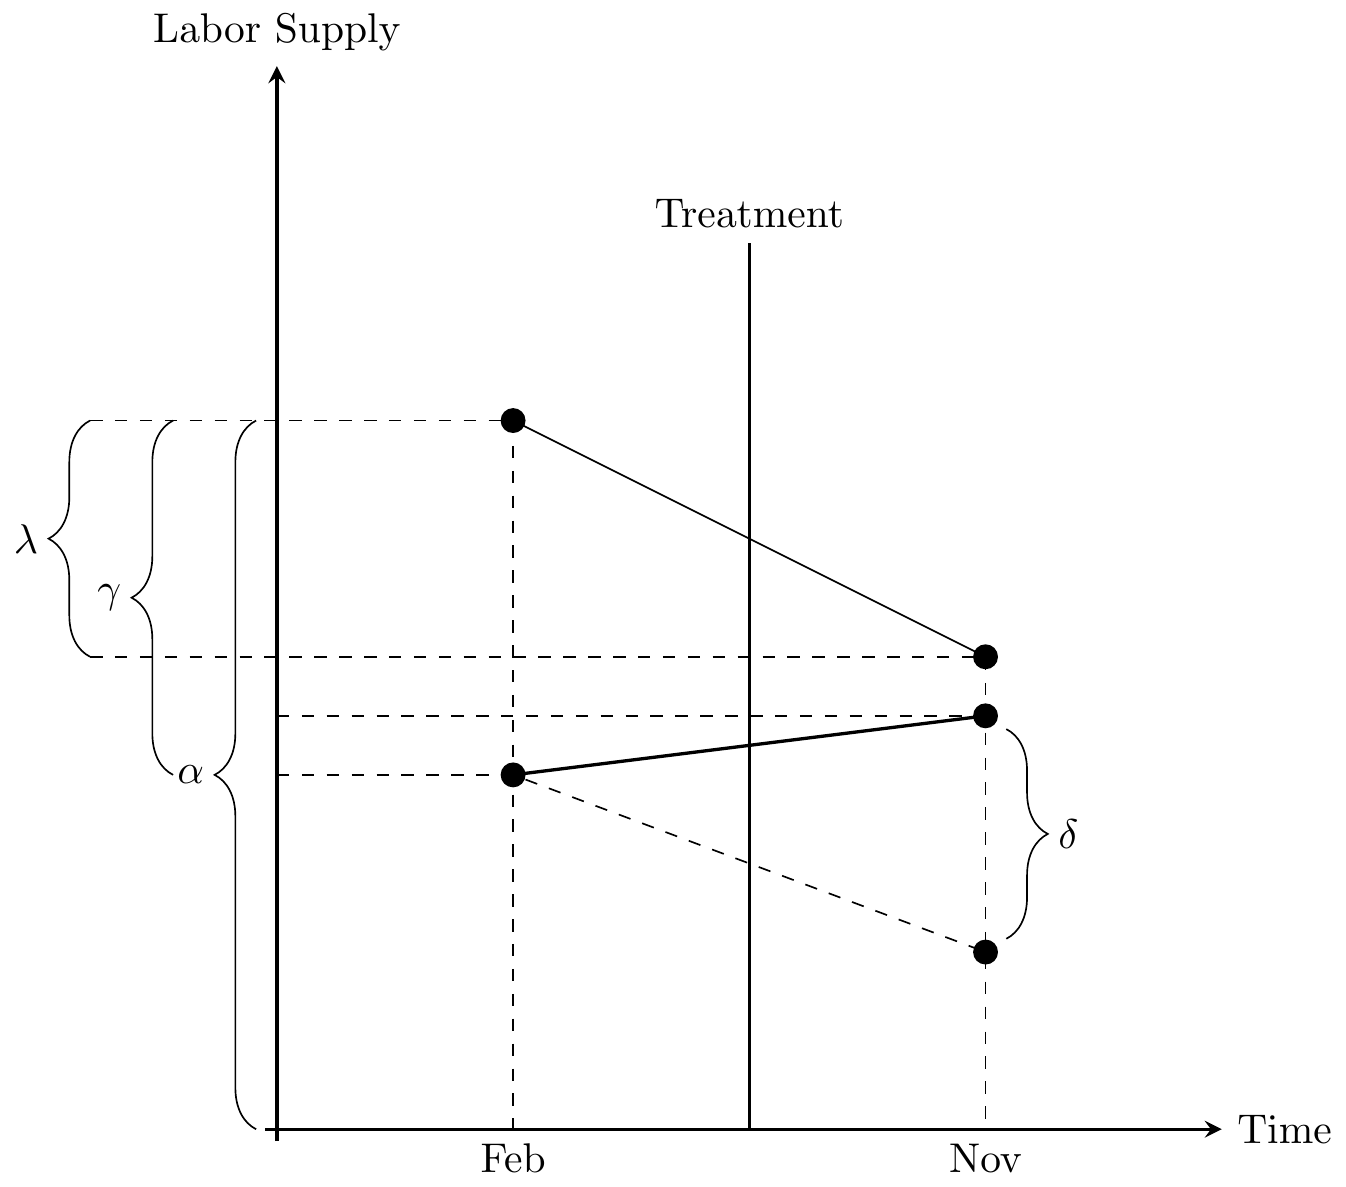
\includegraphics[scale=0.6]{img/fig-dd-diagram-1.png}
\end{figure}
\end{column}

\begin{column}{.45\textwidth}
\begin{itemize}
    \item $\alpha$: Control in pre period

    [PA in Feb.]

    \item $\alpha + \lambda$: Control in post period

    [PA in Nov.]

    \item $\alpha + \gamma$: Treatment in pre period

    [NJ in Feb.]

    \item $\alpha + \gamma + \lambda + \delta$: Treatment in post period

    [NJ in Nov.]
\end{itemize}

The value $\delta$ equals:
\begin{equation*}
    \delta = \EE [Y_{NJ, Post} (1)] - \EE [Y_{NJ, Pre} (0)]
\end{equation*}
Difference between a counterfactual level of employment and the actual level of employment for New Jersey
\end{column}

\end{columns}

\end{frame}

%%%%%%%%%%%%%%%%%%%%%%%%%%%%%%%%%%%%%%%%%%%%%%%%%%%%%%%%%%%%%%%%%%%%%%%%%%%%%%%%
\begin{frame}{Inference in diff-in-diff}

\begin{itemize}
    \item Many studies employing DD strategies use data from many years—not just one pre-treatment and one post-treatment period like Card and Krueger (1994)

    \item The variables of interest in many of these setups only vary at a group level, such as the state, and outcome variables are often serially correlated

    \begin{itemize}
        \item In Card and Krueger (1994), it is very likely for instance that employment in each state is not only correlated within the state but also serially correlated
    \end{itemize}

    \item Bertrand, Duflo, and Mullainathan (2004) point out that the conventional standard errors often severely understate the standard deviation of the estimators, and so standard errors are biased downward, “too small,” and therefore overreject the null hypothesis
\end{itemize}

Bertrand, Duflo, and Mullainathan (2004) propose the following solutions:
\begin{enumerate}
    \item Block bootstrapping standard errors

    \item Aggregating the data into one pre and one post period

    \alert{\item Clustering standard errors at the group level} \emph{(You can just do this one)}

\end{enumerate}


\end{frame}


%%%%%%%%%%%%%%%%%%%%%%%%%%%%%%%%%%%%%%%%%%%%%%%%%%%%%%%%%%%%%%%%%%%%%%%%%%%%%%%%
\begin{frame}{Checking for parallel trends}

Checking for parallel trends is fundamentally untestable
\begin{itemize}
    \item Even if trends were the same before the treatment, there is no guarantee they'd be the same after
    \item That said, you can do intuitive checks to see if this assumption is reasonable
\end{itemize}

\vspace{3ex}
\begin{enumerate}
    \item Plot the raw data, and inspect whether the pre-treatment dynamics of the treatment group differed from that of the control group units

    \item The current way in which authors evaluate the pre-treatment dynamics between a treatment and control group with differential timing is to estimate a regression model that includes treatment leads and lags.
\end{enumerate}


\end{frame}

%%%%%%%%%%%%%%%%%%%%%%%%%%%%%%%%%%%%%%%%%%%%%%%%%%%%%%%%%%%%%%%%%%%%%%%%%%%%%%%%
\begin{frame}{Miller et al. (2019)}

\begin{itemize}
    \item Miller et al. (2019) estimated the effect that Medicaid expansion under the ACA had on population mortality

    \item Their focus is on the near-elderly adults in states with and without the Affordable Care Act Medicaid expansions. They find a 0.13-percentage-point decline in annual mortality as a result of the ACA expansion, which is a 9.3\% reduction over the sample mean
    \begin{itemize}
        \item \textbf{This means the ACA medicaid expansion saved lives}
    \end{itemize}
\end{itemize}

\vspace{2ex}
 Miller et al. (2019) use diff-in-diff:
 \begin{itemize}
      \item Evaluate the pre-treatment leads instead of plotting the raw data by treatment and control
      \item Post-estimation, they plotted regression coefficients with 95\% confidence intervals on their treatment leads and lags
      \item Allows reader to check comparability pre-treatmnet, as well as see post-treatment dynamics
  \end{itemize} 

\begin{equation*}
    Y_{its} = \gamma_s + \lambda_t  + \sum_{\tau = -q}^{-1} \gamma_\tau D_{s\tau}
    + \sum_{\tau=0}^m \delta_\tau D_{s\tau} + x_{ist} + \epsilon_{ist}
\end{equation*}
\begin{itemize}
    \item Regression includes $q$ anticipatory leads and $m$ lags (post-treatment effects)
\end{itemize}
\end{frame}

%%%%%%%%%%%%%%%%%%%%%%%%%%%%%%%%%%%%%%%%%%%%%%%%%%%%%%%%%%%%%%%%%%%%%%%%%%%%%%%%
\begin{frame}{Effect of medicaid expansion on medicaid eligibility}

\begin{figure}
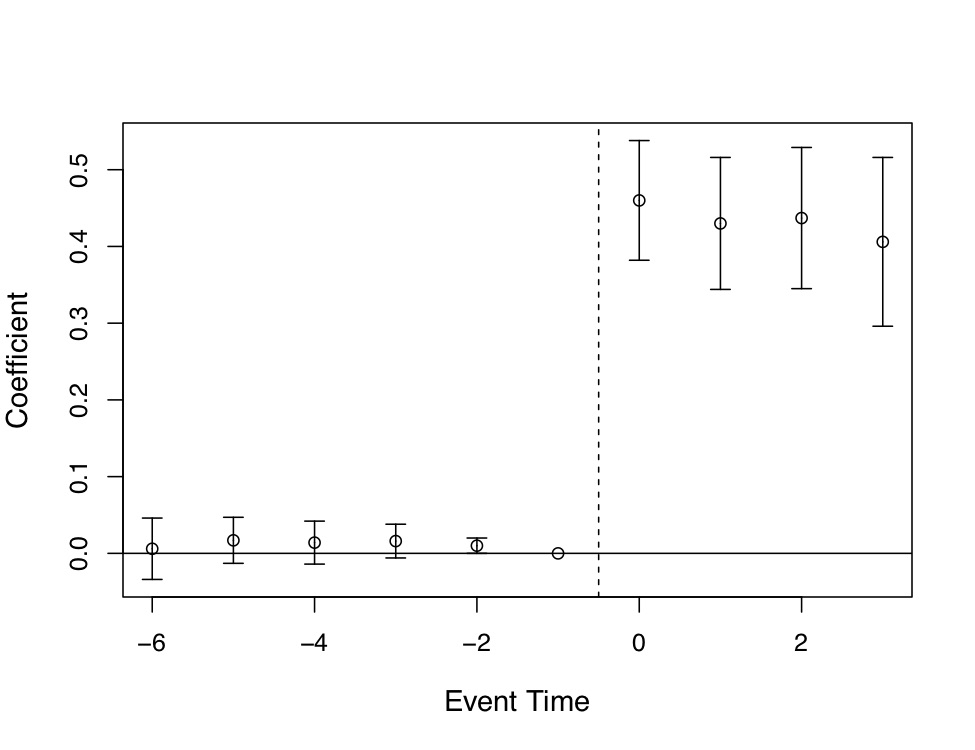
\includegraphics[scale=0.25]{img/fig-9-4.jpg}
\end{figure}

\end{frame}

%%%%%%%%%%%%%%%%%%%%%%%%%%%%%%%%%%%%%%%%%%%%%%%%%%%%%%%%%%%%%%%%%%%%%%%%%%%%%%%%
\begin{frame}{Effect of medicaid expansion on medicaid coverage}

\begin{figure}
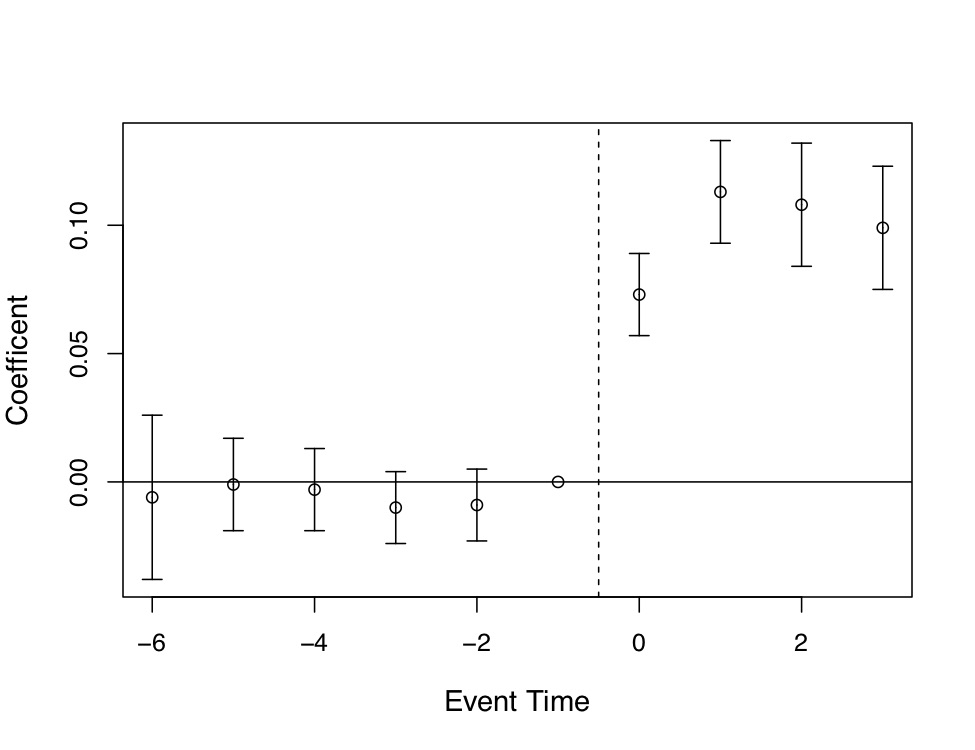
\includegraphics[scale=0.25]{img/fig-9-5.jpg}
\end{figure}

\end{frame}

%%%%%%%%%%%%%%%%%%%%%%%%%%%%%%%%%%%%%%%%%%%%%%%%%%%%%%%%%%%%%%%%%%%%%%%%%%%%%%%%
\begin{frame}{Effect of medicaid expansion on percentage of the uninsured population}

\begin{figure}
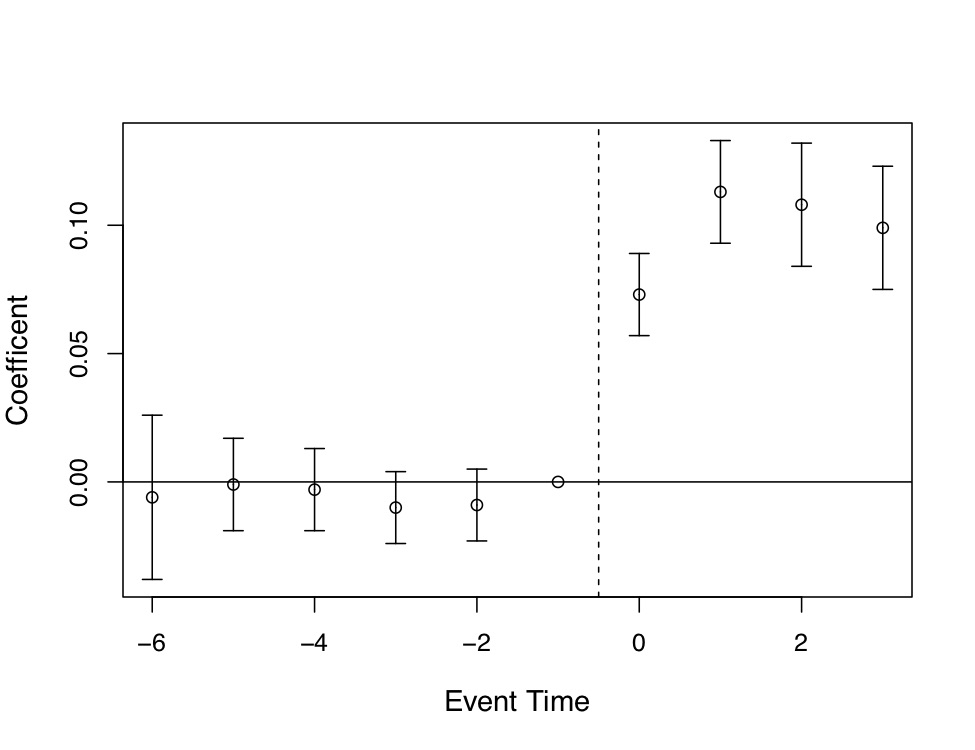
\includegraphics[scale=0.25]{img/fig-9-5.jpg}
\end{figure}

\end{frame}

%%%%%%%%%%%%%%%%%%%%%%%%%%%%%%%%%%%%%%%%%%%%%%%%%%%%%%%%%%%%%%%%%%%%%%%%%%%%%%%%
\begin{frame}{Effect of medicaid expansion on mortality}

\begin{figure}
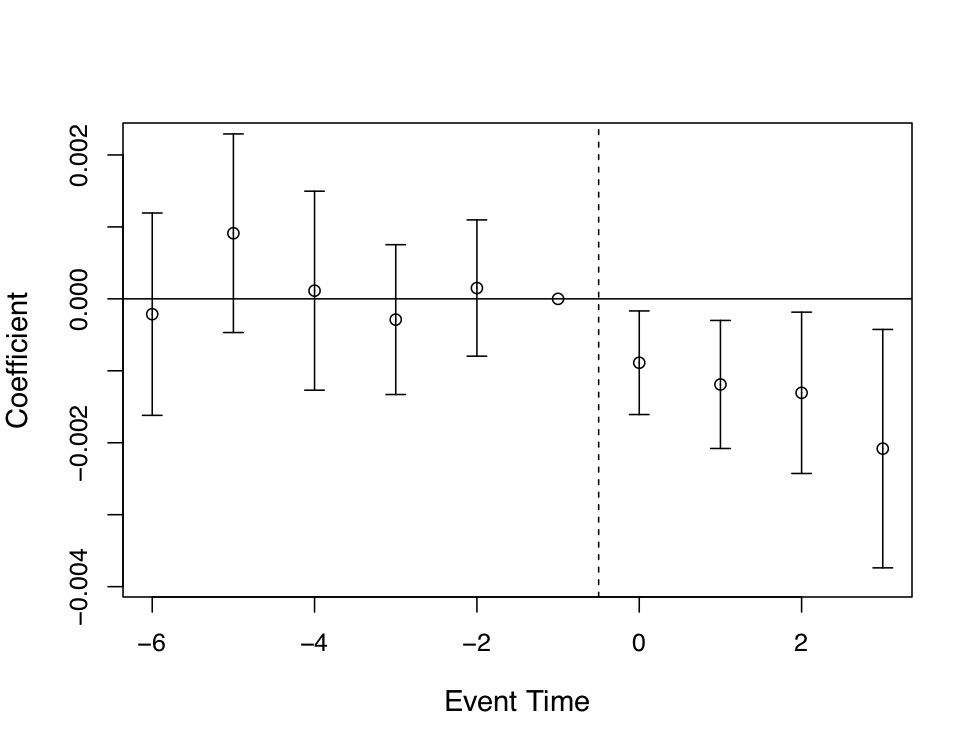
\includegraphics[scale=0.25]{img/fig-907.jpg}
\end{figure}

\end{frame}

%%%%%%%%%%%%%%%%%%%%%%%%%%%%%%%%%%%%%%%%%%%%%%%%%%%%%%%%%%%%%%%%%%%%%%%%%%%%%%%%
\begin{frame}{Diff-in-diff estimation}

Go through example here: \url{https://mixtape.scunning.com/09-difference_in_differences\#abortion-legalization-and-long-term-gonorrhea-incidence}
\begin{itemize}
    \item Python code available on my github: \url{https://github.com/tara-sullivan/econ726-notebooks/blob/main/notebooks/08-diff-in-diff.ipynb}
    \item See published paper here (Table 3): \url{https://www.scunning.com/files/cunningham-and-cornwell.pdf}
\end{itemize}

\end{frame}



\end{document}
